\usetikzlibrary{shapes, arrows.meta, positioning, fit, decorations.pathreplacing,
decorations.pathmorphing, decorations.shapes, calc}

\pgfdeclarelayer{background}
\pgfdeclarelayer{middle}
\pgfsetlayers{background,middle,main}

\tikzset{dada2/.style={draw, fill=green!10, align=center}}
\tikzset{vsearch/.style={draw, fill=red!20, align=center}}
\tikzset{usearch/.style={draw, fill=magenta!10, align=center}}
\tikzset{cutadapt/.style={draw, fill=cyan!10, align=center}}
\tikzset{protax/.style={draw, fill=blue!15, align=center}}
\tikzset{protax_or_vsearch/.style={draw, shade, right color=blue!15, left color=red!20, align=center}}
\tikzset{protax_or_usearch/.style={draw, shade, right color=blue!15, left color=magenta!10, align=center}}
\tikzset{infernal/.style={draw, fill=orange!15, align=center}}
\tikzset{new/.style={draw, fill=yellow!10, align=center}}
\tikzset{data/.style={align=center}}
\tikzset{key/.style={minimum width=35mm}}

% \tikzset{parallel/.style={dotted, line width=1pt}}
\tikzset{parallel/.style={fill=gray!20, rounded corners}}
\tikzset{paired reads/.style={line width = 1pt, double distance=0.5pt,decorate, decoration={snake, amplitude=0.75pt, segment length = 3pt, post=lineto, post length=2mm}}}
\tikzset{single reads/.style={decorate, decoration={snake, amplitude=0.75pt, segment length = 3pt, post=lineto, post length=2mm}}}
\tikzset{table/.style={line width=1pt}}
\tikzset{taxonomy/.style={double distance=0.5pt}}

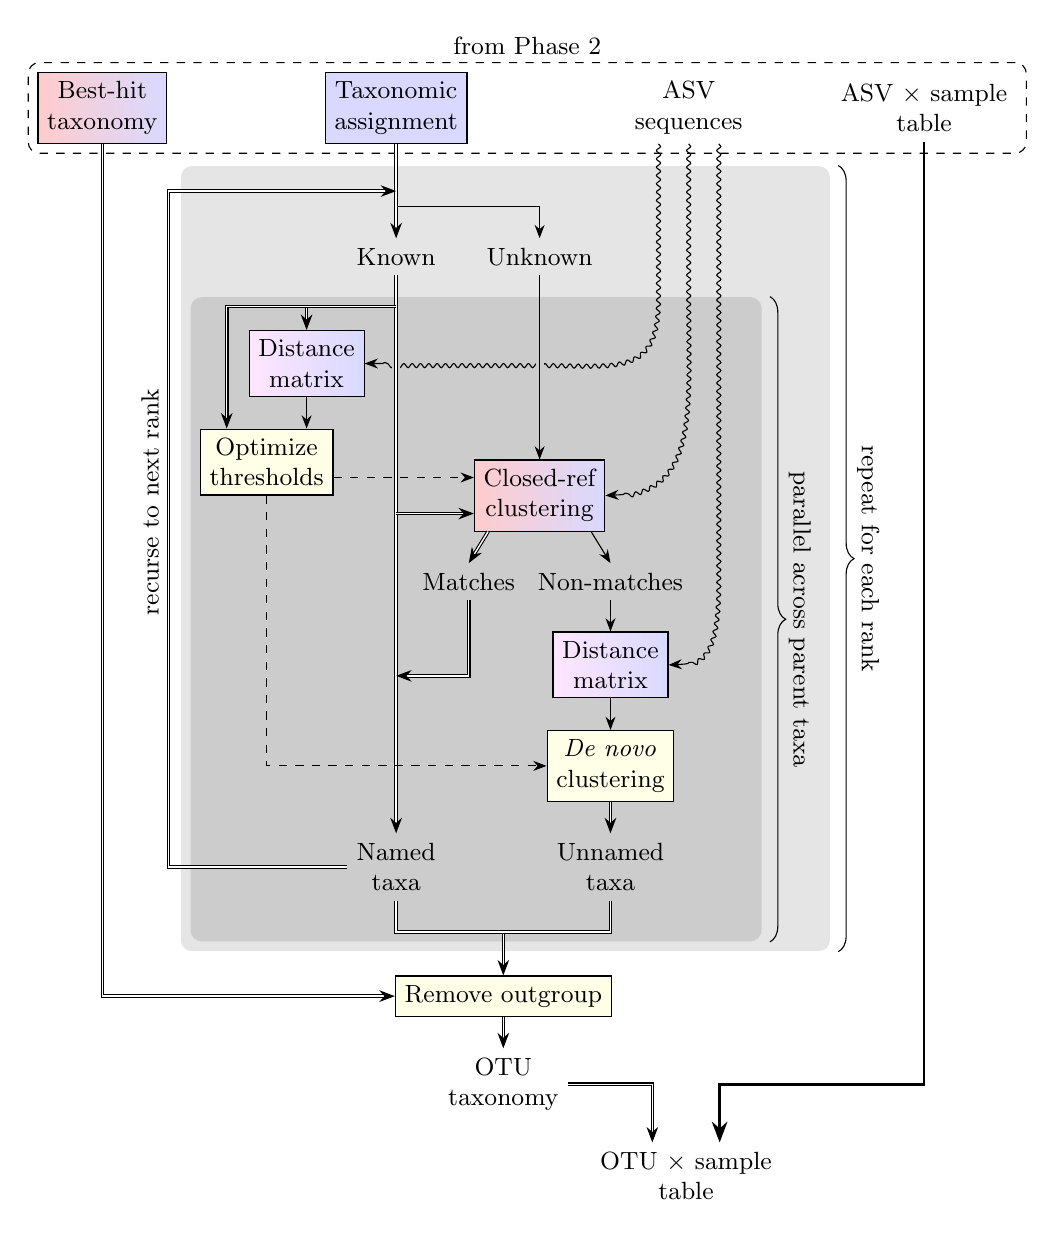
\begin{tikzpicture}[font=\small,node distance=4mm]
\node[protax] (protax) {Taxonomic \\ assignment};
\node[left=20mm of protax, protax_or_vsearch] (besthit) {Best-hit \\ taxonomy};
\node[right = 20mm of protax, data] (nonspike) {ASV \\ sequences};
\node[right = 10mm of nonspike, data] (ASV) {ASV $\times$ sample \\ table};

\node[fit=(protax) (besthit) (nonspike) (ASV), draw, rounded corners, dashed] (phase2) {};
\node[anchor=south, above=1mm of phase2.north, anchor=base] {from Phase 2};

\coordinate[below = of $(nonspike.south-|protax)$] (p4);
\coordinate[below = of p4] (p5);
\node[below = of p5, data] (known) {Known};
\node[right = of known, data] (unknown) {Unknown};
\coordinate[below = of known](p8);
\node[below left = 3mm and 4mm of p8, protax_or_usearch] (calibmx) {Distance \\ matrix};
\node[below = of calibmx, new, anchor=40] (optimize) {Optimize \\ thresholds};
% \coordinate[below=of optimize] (p9);
%\node[right=of unknown, align = center, color=orange!60] (thresholds) {Optimized \\ thresholds};
\node[protax_or_vsearch] (closedref) at (optimize.south-|unknown) {Closed-ref \\ clustering};
\node[below right = 4mm and 9mm of closedref.south, data, anchor = north] (mismatch) {Non-matches};
\node[below left = 4mm and 9mm of closedref.south, data, anchor = north] (match) {Matches};

% \coordinate[right=4mm of DADA2.east] (p1);
%\node[draw, below=of protax, align = center, fill=green!10]
\node[below=of mismatch, protax_or_usearch] (distmx) {Distance \\ matrix};
\node[below=of distmx, new] (cluster) {\emph{De novo} \\ clustering};
\node[below=of cluster, data] (unnamed) {Unnamed\\taxa};
\node[data] (named) at (known |- unnamed) {Named\\taxa};
\coordinate (p3) at (nonspike.east |- cluster);
\coordinate[above = 20mm of named.north] (p6);
\coordinate[below=of $(named.south)!.5!(unnamed.south)$] (p7);
% \node[draw,fit=(closedref) (match) (cluster) (named) (distmx) (p7)] (rank) {};
% \node[anchor = north east, align=center] at (rank.north east) (ranklabel) {Repeat \\ for each \\ rank};
\node[below=of p7, yshift = -1.5mm, new] (fungi) {Remove outgroup};
\node[below=of fungi, data] (taxonomy) {OTU \\ taxonomy};
\coordinate[below right = of taxonomy] (p11);
\node[below right=of taxonomy, data] (OTU) {OTU $\times$ sample \\ table};

\begin{pgfonlayer}{middle}
\node[parallel, fit=(named) (cluster) (closedref) (p3) (p7) (distmx) (p8) (optimize), fill=gray!40] (parent) {};
\end{pgfonlayer}
\draw[decorate, decoration={brace, raise = 1mm, amplitude=2mm}] (parent.north east) -- (parent.south east) ;
\node[rotate=-90,right=4mm of parent, anchor=base, align=center] (parentlabel){parallel across parent taxa};

\begin{pgfonlayer}{background}
\node[parallel, fit=(parent) (parentlabel) (p4)] (rank) {};
\end{pgfonlayer}
\draw[decorate, decoration={brace, raise = 1mm, amplitude=2mm}] (rank.north east) -- (rank.south east) ;
\node[rotate=-90,right=4mm of rank, anchor=base, align=center] (ranklabel){repeat for each rank};

\draw[-Stealth, single reads] (nonspike.310) -- (nonspike.310|-mismatch) .. controls +(270:10mm) and +(0:4mm) .. (distmx.east);
\draw[-Stealth, single reads] (nonspike.south) -- (nonspike|-parent.north) .. controls +(270:15mm) and +(0:12mm) .. (closedref.east);
\draw[-Stealth, single reads] (nonspike.230) -- (nonspike.230|-parent.north) .. controls +(270:10mm) and +(0:10mm) .. (unknown|-calibmx) -- (calibmx);


\draw[-Stealth] (p5) -| (unknown.north);
\draw[-Stealth,taxonomy] (protax) -- (p5) -| (known.north);
\draw[gray!40, line width=1mm] (unknown|-parent.north) -- (closedref);
\draw[-Stealth] (unknown) edge (closedref);
\draw[-Stealth] (closedref.325) -- (mismatch.north);
\draw[-Stealth, taxonomy] (closedref.215) -- (match.north);
\draw[-Stealth] (mismatch) edge (distmx);
\draw[-Stealth] (distmx) edge (cluster);
\draw[gray!40, line width=1mm] (p8) -- (p6);
\draw[-Stealth,taxonomy] (known) -- (p8) -| (named.north);
\draw[-Stealth,taxonomy] (p8) -| (calibmx);
\draw[-Stealth] (calibmx) -- (optimize.north-|calibmx);
\draw[-Stealth,taxonomy] (p8-|calibmx) -| (optimize.140);
\draw[-Stealth, taxonomy] ($(named|-closedref.south)!0.5!(named|-optimize.south)$) -- ($(closedref.south west)!0.5!(closedref.west|-optimize.south)$);
\draw[-Stealth,dashed] ($(optimize.south east)!0.5!(optimize.east|-closedref.north)$) -- ($(optimize.south-|closedref.west)!0.5!(closedref.north west)$);
\draw[-Stealth,dashed] (optimize) |- (cluster);
\draw[-Stealth,taxonomy] (cluster) -- (unnamed);
\draw[-Stealth,taxonomy] (match) |- (p6);
\draw[-Stealth,taxonomy] (named) |- (p7) -- (fungi);
\draw[-Stealth,taxonomy] (named) -- (named-|rank.west) -- +(-1.5mm,0) |- ($(p4)!0.5!(p5)$) node[pos=0.27,above,sloped]{recurse to next rank};
\draw[-Stealth,taxonomy] (besthit) |- (fungi);
\draw[taxonomy] (unnamed) |- (p7);
\draw[-Stealth,taxonomy] (fungi) -- (taxonomy);
\draw[-Stealth,taxonomy] (taxonomy) -| (OTU.135);
\coordinate[below = of ASV] (p12);
\coordinate[left = of calibmx] (p10);
\draw[-Stealth, table] (ASV) |- (ASV|-taxonomy) -| (OTU.45);
\end{tikzpicture}
